% =============================================================
% ROS 2 SLAM & RL Resource Management Presentation
% =============================================================
\documentclass[aspectratio=169]{beamer}

% --- Theme Selection ---
\usetheme{Madrid}
\usecolortheme{dolphin} % Blue theme (clean and academic)
% \usecolortheme{beaver} % Option: Red theme if you prefer

% --- Packages ---
\usepackage{graphicx}
\usepackage{booktabs} % For nicer tables
\usepackage{tikz}
\usetikzlibrary{shapes, arrows, positioning, fit, calc, decorations.pathmorphing, shadows}
\usepackage{amsmath}

% --- Title Information ---
\title[ROS 2 Resource Mgmt via RL]{ROS 2 SLAM Resource Management \\ using Reinforcement Learning}
\subtitle{Analysis under CPU Contention in Simulation}
\author[Team Name]{
    \textbf{Group 19} \\
    \and
    Kieu Son Tung \and Nguyen Phu An \and Nguyen Thanh Lam \and Pham Chi Bang 
}
\institute[HUST]{
    Hanoi University of Science and Technology (HUST) \\
    \textit{Class: DSAI-02-K68}
}
\date{\today}

% --- Begin Presentation ---
\begin{document}

% Slide 1: Title
\begin{frame}
    \titlepage
\end{frame}

% Slide 2: Table of Contents
\begin{frame}{Outline}
    \tableofcontents
\end{frame}

% =============================================================
% Section 1: Introduction to ROS 2
% =============================================================
\section{Introduction to ROS 2}
\begin{frame}{1. Introduction to ROS 2}
    \begin{columns}
        \column{0.6\textwidth}
        \textbf{Robot Operating System 2 (ROS 2)} is the industry standard middleware for robotics.
        \vspace{0.5cm}
        \begin{itemize}
            \item \textbf{Nodes:} Independent processes performing specific tasks (e.g., Sensing, Planning, Actuation).
            \item \textbf{Topics:} Publish/Subscribe mechanism for data exchange.
            \item \textbf{SLAM Toolbox:} A popular package for 2D Simultaneous Localization and Mapping.
        \end{itemize}
        
        \column{0.4\textwidth}
        \centering
        % Placeholder for ROS Logo or simple graph
        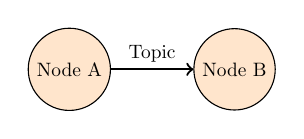
\begin{tikzpicture}[node distance=1.5cm, auto, scale=0.7, transform shape]
            \node[draw, circle, fill=orange!20] (n1) {Node A};
            \node[draw, circle, fill=orange!20, right=of n1] (n2) {Node B};
            \draw[->, thick] (n1) -- node[above] {Topic} (n2);
        \end{tikzpicture}
        \vspace{1cm}
        \begin{block}{Key Feature}
            ROS 2 uses DDS (Data Distribution Service) for real-time communication.
        \end{block}
    \end{columns}
\end{frame}

% =============================================================
% Section 2: Problem Statement
% =============================================================
\section{Problem Statement}
\begin{frame}{2. Problem Statement: Resource Contention}
    \textbf{The Challenge:}
    \begin{itemize}
        \item ROS 2 nodes operate as independent OS processes.
        \item On hardware with limited resources (CPU/RAM), nodes compete for execution time.
    \end{itemize}
    
    \vspace{0.5cm}
    \pause
    
    \textbf{The Symptom:}
    \begin{alertblock}{Without Management}
        When background tasks (image processing, data logging) spike:
        \begin{enumerate}
            \item \textbf{Starvation:} Critical SLAM nodes lose CPU cycles.
            \item \textbf{Latency:} Topic messages (\texttt{/scan}) are delayed.
            \item \textbf{Failure:} Map drift, ghost artifacts, and navigation failure.
        \end{enumerate}
    \end{alertblock}
    
    \vspace{0.3cm}
    \centering
    $\rightarrow$ \textbf{Need for an Intelligent Resource Manager.}
\end{frame}


% --- Slide: Map Drift Visualization ---
\begin{frame}{Visualizing the Problem: Map Drift}
    \centering
    \textbf{Effect of CPU Starvation on Mapping}
    
    \vspace{0.5cm}
    
    % Thay đổi kích thước width=0.7 tùy theo tỉ lệ ảnh của bạn
    \includegraphics[width=0.75\linewidth]{drift.png}
    
    \vspace{0.5cm}
    \begin{block}{Observation}
        Due to high jitter in \texttt{/scan} and delayed TF transforms, the robot rotates physically but the map update lags behind, creating \textbf{"ghost walls"} and angular misalignment.
    \end{block}
\end{frame}
% =============================================================
% Section 3: Experimental Setup
% =============================================================
\section{Experimental Setup}
\begin{frame}{3. Experimental Setup}
    \textbf{Environment:}
    \begin{itemize}
        \item \textbf{Robot:} TurtleBot3 (Burger) in Gazebo Simulation.
        \item \textbf{Stress Injector:} \texttt{cpu\_hog} nodes (consume 60-100\% CPU).
        \item \textbf{Metrics:} Jitter ($\sigma_t$), Throughput (Hz), Map Quality.
    \end{itemize}

    \vspace{0.2cm}
    
    % TikZ Diagram simplified for Slide
    \centering
    \resizebox{0.75\linewidth}{!}{
    % \begin{tikzpicture}[
    %     node distance=1cm and 1cm,
    %     box/.style={draw, rounded corners, minimum width=2cm, minimum height=1cm, align=center, font=\bfseries\sffamily},
    %     sim/.style={box, fill=blue!10, draw=blue!70},
    %     ros/.style={box, fill=orange!10, draw=orange!70},
    %     stress/.style={box, fill=red!10, draw=red!70, dashed},
    %     arrow/.style={->, >=stealth, thick, color=darkgray}
    % ]
    %     \node[sim] (gaz) {Gazebo};
    %     \node[ros, right=of gaz] (bridge) {Bridge};
    %     \node[ros, right=of bridge] (slam) {SLAM};
    %     \node[stress, above=0.5cm of slam] (hog) {CPU Hog};
    %     \node[box, fill=green!10, below=0.5cm of bridge] (rl) {RL Agent};

    %     \draw[arrow] (gaz) -- (bridge);
    %     \draw[arrow] (bridge) -- (slam);
    %     \draw[->, decorate, decoration={snake}, red, thick] (hog) -- (slam);
    %     \draw[arrow, dashed] (rl) -| node[pos=0.2, above] {Control} (slam);
    %     \draw[arrow, dashed] (bridge) |- (rl);
    % \end{tikzpicture}
    }
\end{frame}

% =============================================================
% Section 4: RL, Q-Learning and Bandit
% =============================================================
\section{RL, Q-Learning and Bandit}
\begin{frame}{4. Reinforcement Learning Approach}
    We treat Resource Management as a decision-making problem.
    
    \begin{columns}[T]
        \column{0.5\textwidth}
        \textbf{Multi-Armed Bandit (MAB)}
        \begin{itemize}
            \item \textit{Stateless}: Does not consider current CPU load.
            \item Algorithm: $\epsilon$-greedy.
            \item Action: Fix Priority.
            \item \textit{Pro:} Simple. \textit{Con:} Ignores context.
        \end{itemize}

        \column{0.5\textwidth}
        \textbf{Q-Learning (MDP)}
        \begin{itemize}
            \item \textit{State-Aware}: State $S \in \{Safe, Warning, Critical\}$.
            \item Update Rule:
            {\footnotesize $$Q(s,a) \leftarrow Q(s,a) + \alpha [r + \gamma \max Q(s',a') - Q(s,a)]$$}
            \item \textit{Pro:} Anticipatory behavior.
        \end{itemize}
    \end{columns}

    \vspace{1cm}
    \centering
    \textbf{Action Space:} \{Normal Priority, High Priority SLAM, Throttle Hog\} \\
    \textbf{Reward:} $+1$ if Jitter $< 50ms$, else $-1$.
\end{frame}

% =============================================================
% Section 5: Experimental Results
% =============================================================
\section{Experimental Results}
\begin{frame}{5. Experimental Results}
    \textbf{Scenario:} High Contention (2 Hog Processes active).
    
    \begin{table}
        \centering
        \begin{tabular}{l c c c}
            \toprule
            \textbf{Method} & \textbf{Scan Rate (Hz)} & \textbf{Jitter (ms)} & \textbf{Map Quality} \\
            \midrule
            Baseline (None) & $1 \pm 0.8$ & $120$ & \textcolor{red}{Poor (Drift)} \\
            Rule-Based & $1.1 \pm 0.5$ & $75$ & Medium \\
            Bandit (MAB) & $1.3 \pm 0.2$ & $48$ & Medium-High \\
            \textbf{Q-Learning} & $\mathbf{1.5 \pm 0.2}$ & $\mathbf{25}$ & \textcolor{green!60!black}{\textbf{High (Stable)}} \\
            \bottomrule
        \end{tabular}
        \caption{Performance metrics comparison over 120s episode.}
    \end{table}

    \begin{itemize}
        \item \textbf{Baseline:} SLAM starves, leading to broken maps.
        \item \textbf{Q-Learning:} Automatically preempts "Hog" processes when Jitter rises, maintaining 4.8Hz stability.
    \end{itemize}
\end{frame}

% --- Slide: Q-Learning vs Bandit Comparison ---
\begin{frame}{Performance Comparison: Bandit vs. Q-Learning}
    \centering
    \textbf{Learning Convergence \& Stability}
    \vspace{0.3cm}

    \begin{columns}[T] % T = align top
        % Cột trái: Bandit
        \column{0.48\textwidth}
        \centering
        \textbf{1. Bandit ($\epsilon$-greedy)} \\
        \vspace{0.2cm}
        \fbox{\includegraphics[width=\linewidth]{bandit.png}}
        \vspace{0.2cm}
        \footnotesize{\textit{High oscillation. The agent struggles to stick to an optimal policy in changing load states.}}

        % Cột phải: Q-Learning
        \column{0.48\textwidth}
        \centering
        \textbf{2. Q-Learning (State-Aware)} \\
        \vspace{0.2cm}
        \fbox{\includegraphics[width=\linewidth]{Q.png}}
        \vspace{0.2cm}
        \footnotesize{\textit{Stable convergence. The agent learns to distinguish between 'Safe' and 'Critical' states effectively.}}
    \end{columns}
\end{frame}

% =============================================================
% Section 6: Limitations
% =============================================================
\section{Limitations}
\begin{frame}{6. Limitations}
    Despite positive results, several factors impact the fidelity:

    \begin{enumerate}
        \item \textbf{WSL2 Virtualization:}
            \begin{itemize}
                \item Running on Windows Subsystem for Linux (WSL2) introduces scheduler noise from the Windows host.
                \item Not a true "Real-Time" kernel (RT-Preempt).
            \end{itemize}
        
        \item \textbf{Resource Constraints:}
            \begin{itemize}
                \item Limited to virtual cores; difficult to isolate CPU affinity strictly compared to bare-metal Linux.
            \end{itemize}

        \item \textbf{System Complexity:}
            \begin{itemize}
                \item ROS 2 Middleware (DDS) has its own internal buffering which RL does not directly control.
            \end{itemize}
    \end{enumerate}
\end{frame}

% =============================================================
% Conclusion
% =============================================================
\begin{frame}{}
    \centering
    
    \vspace{1cm}
    \textbf{Thank you for listening!} \\
\end{frame}

\end{document}
